\documentclass[12pt,a4paper,UTF8]{ctexart}
\usepackage{graphicx}
\usepackage{amsmath}
\usepackage{amssymb}
\usepackage{cite}
\usepackage[ntheorem]{empheq}
\usepackage{enumitem}
\usepackage{fullpage}
\usepackage{tocbibind}
\usepackage[bookmarksopen=true,colorlinks,linkcolor=black]{hyperref}
\usepackage{cellspace}
\usepackage{listings}
\usepackage{color}
\usepackage{epstopdf}
\usepackage{subfigure}
\usepackage{algorithm}
\usepackage{algorithmicx}
\usepackage{algpseudocode}
\usepackage{lipsum}
\usepackage[thmmarks,amsmath]{ntheorem}



\theoremstyle{nonumberplain}

\theoremheaderfont{\bfseries}

\theorembodyfont{\normalfont}

\theoremsymbol{$\square$}

\newtheorem{Proof}{\hskip 2em 证明}


\makeatletter
\newenvironment{breakablealgorithm}
  {% \begin{breakablealgorithm}
   \begin{center}
     \refstepcounter{algorithm}% New algorithm
     \hrule height.8pt depth0pt \kern2pt% \@fs@pre for \@fs@ruled
     \renewcommand{\caption}[2][\relax]{% Make a new \caption
       {\raggedright\textbf{\ALG@name~\thealgorithm} ##2\par}%
       \ifx\relax##1\relax % #1 is \relax
         \addcontentsline{loa}{algorithm}{\protect\numberline{\thealgorithm}##2}%
       \else % #1 is not \relax
         \addcontentsline{loa}{algorithm}{\protect\numberline{\thealgorithm}##1}%
       \fi
       \kern2pt\hrule\kern2pt
     }
  }{% \end{breakablealgorithm}
     \kern2pt\hrule\relax% \@fs@post for \@fs@ruled
   \end{center}
  }
\makeatother
\renewcommand{\algorithmicrequire}{\textbf{Input:}}  % Use Input in the format of Algorithm
\renewcommand{\algorithmicensure}{\textbf{Output:}} % Use Output in the format of Algorithm
\usepackage{longtable}

\usepackage{float}
\definecolor{gray}{rgb}{0.5,0.5,0.5}
\definecolor{dkgreen}{rgb}{.068,.578,.068}
\definecolor{dkpurple}{rgb}{.320,.064,.680}

% set Matlab styles
\lstset{
   language=Matlab,
   numbers=left,
   keywords={break,case,catch,continue,else,elseif,end,for,function,
      global,if,otherwise,persistent,return,switch,try,while},
   basicstyle=\ttfamily,
   keywordstyle=\color{blue}\bfseries,
   commentstyle=\color{dkgreen},
   stringstyle=\color{dkpurple},
   backgroundcolor=\color{white},
   breaklines=true,
   tabsize=4,
   showspaces=false,
   showstringspaces=false,
}

\begin{document}
\CJKfamily{zhkai}


\begin{center}
    \textbf{作业二}\\
    \textbf{姓名 胡毅翔 ~~ 学号 PB18000290 ~~ 日期 2021年5月29日}\\
\end{center}

\begin{center}
    \fbox{
        \begin{minipage}{40em}
            \vspace{5cm}
            \hspace{20cm}
        \end{minipage}}
\end{center}
\vspace{1cm}

\begin{enumerate}
    \item[第一题] 本题考虑对于定义在 $[-1,1]$ 上的一个光滑函数 $f(x)$ 的三次样条插值的使用。下面 所说的误差都是指绝对误差。
          \begin{enumerate}\item(10分)仿照课堂笔记或课本推导出关于额外给定边界点处(即-1和1)三
                    次样条插值多项式的一次导数值时其在各插值点上的二次导数值应该满足的
                    线性方程组。请给出推导过程。
                    \par 解:
                    \par 记 $S(x)$ 在区间 $\left[x_{i}, x_{i+1}\right]$ 上的表达式为 $S_{i}(x), S(x)$ 是三次多项式, $S^{\prime \prime}(x)$ 是 线性函数, 用插值点 $\left\{\left(x_{i}, S^{\prime \prime}\left(x_{i}\right)\right),\left(x_{i+1}, S^{\prime \prime}\left(x_{i+1}\right)\right)\right\}$ 作线性插值, 记 $S^{\prime \prime}\left(x_{i}\right)=M_{i}$,
                    $S^{\prime \prime}\left(x_{i+1}\right)=M_{i+1}$
                    $$
                        S_{i}^{\prime \prime}(x)=\frac{x-x_{i+1}}{x_{i}-x_{i+1}} M_{i}+\frac{x-x_{i}}{x_{i+1}-x_{i}} M_{i+1}, \quad x_{i} \leqslant x \leqslant x_{i+1}
                    $$
                    对 $S^{\prime \prime}(x)$ 积分两次, 记 $h_{i}=x_{i+1}-x_{i}$,
                    $$
                        \begin{aligned}
                            S(x) & =S_{i}(x)=\frac{\left(x_{i+1}-x\right)^{3}}{6 h_{i}} M_{i}+\frac{\left(x-x_{i}\right)^{3}}{6 h_{i}} M_{i+1}+c x+d                                \\
                                 & =\frac{\left(x_{i+1}-x\right)^{3}}{6 h_{i}} M_{i}+\frac{\left(x-x_{i}\right)^{3}}{6 h_{i}} M_{i+1}+C\left(x_{i+1}-x\right)+D\left(x-x_{i}\right)
                        \end{aligned}
                    $$
                    将 $S\left(x_{i}\right)=y_{i}, S\left(x_{i+1}\right)=y_{i+1}$ 代入上式解出
                    $$
                        C=\frac{y_{i}}{h_{i}}-\frac{h_{i} M_{i}}{6}, \quad D=\frac{y_{i+1}}{h_{i}}-\frac{h_{i} M_{i+1}}{6}
                    $$
                    \begin{equation}\label{eq1}
                        \begin{aligned}
                            S(x)= & \frac{\left(x_{i+1}-x\right)^{3} M_{i}+\left(x-x_{i}\right)^{3} M_{i+1}}{6 h_{i}}+\frac{\left(x_{i+1}-x\right) y_{i}+\left(x-x_{i}\right) y_{i+1}}{h_{i}} \\
                                  & -\frac{h_{i}}{6}\left[\left(x_{i+1}-x\right) M_{i}+\left(x-x_{i}\right) M_{i+1}\right], \quad x \in\left[x_{i}, x_{i+1}\right]
                        \end{aligned}\end{equation}

                    在内结点 $x_{i}$, 由 $S_{i}^{\prime}\left(x_{i}\right)=S_{i-1}^{\prime}\left(x_{i}\right)$ 可得到
                    \begin{equation}\label{eq2}
                        f\left(x_{i}, x_{i+1}\right)-\frac{h_{i}}{3} M_{i}-\frac{h_{i}}{6} M_{i+1}=f\left(x_{i-1}, x_{i}\right)+\frac{h_{i-1}}{6} M_{i-1}+\frac{h_{i-1}}{3} M_{i}
                    \end{equation}
                    整理后得到
                    \begin{equation}\label{eq3}
                        \mu_{i} M_{i-1}+2 M_{i}+\lambda_{i} M_{i+1}=d_{i}, \quad i=1,2, \cdots, n-1
                    \end{equation}
                    其中
                    $$
                        \begin{array}{c}
                            \lambda_{i}=\frac{h_{i}}{h_{i}+h_{i-1}}, \quad \mu_{i}=1-\lambda_{i} \\
                            d_{i}=\frac{6}{h_{i}+h_{i-1}}\left(\frac{y_{i+1}-y_{i}}{h_{i}}-\frac{y_{i}-y_{i-1}}{h_{i-1}}\right)=6 f\left(x_{i-1}, x_{i}, x_{i+1}\right)
                        \end{array}
                    $$
                    式 \ref{eq2} 称为样条插值的 $M$ 关系方程组,解方程组 \ref{eq2} 得到 $\left\{M_{i}, i=\right.$ $\left.1,2, \cdots, M_{n-1}\right\}$, 再加上两个端点条件, 满足端点条件的样条插值函数 $S(x)$ 在 $\left[x_{i},\right.$, $\left.x_{i+1}\right]$ 上的表达就是式 \ref{eq1}.
                    \par 给定 $S^{\prime}\left(x_{0}\right)=m_{0}, S^{\prime}\left(x_{n}\right)=m_{n}$ 的值, 将 $S^{\prime}\left(x_{0}\right)=m_{0}, S^{\prime}\left(x_{n}\right)=m_{n}$ 的值分
                    别代入 $S^{\prime}(x)$ 在 $\left[x_{0}, x_{1}\right],\left[x_{n-1}, x_{n}\right]$ 中的表达式, 得到另外两个方程:
                    $$
                        \begin{array}{c}
                            2 M_{0}+M_{1}=\frac{6}{h_{0}}\left[f\left[x_{0}, x_{1}\right]-m_{0}\right]=d_{0} \\
                            M_{n-1}+2 M_{n}=\frac{6}{h_{n-1}}\left[m_{n}-f\left[x_{n-1}, x_{n}\right]\right]=d_{n}
                        \end{array}
                    $$
                    得到 $n+1$ 个未知量, $n+1$ 个方程组
                    $$
                        \left[\begin{array}{cccccc}
                                2        & 1        &             &             &        &               \\
                                \mu _{1} & 2        & \lambda_{1} &             &        &               \\
                                         & \mu _{2} & 2           & \lambda_{2} &        &               \\
                                         &          & \ddots      & \ddots      & \ddots &               \\
                                         &          &             & \mu _{n-2}  & 2      & \lambda_{n-1} \\
                                         &          &             &             & 1      & 2
                            \end{array}\right]\left[\begin{array}{c}
                                M_{0}   \\
                                M_{1}   \\
                                M_{2}   \\
                                \vdots  \\
                                M_{n-1} \\
                                M_{n}
                            \end{array}\right]=\left[\begin{array}{c}
                                d_{0}   \\
                                d_{1}   \\
                                d_{2}   \\
                                \vdots  \\
                                d_{n-1} \\
                                d_{n}
                            \end{array}\right]
                    $$
              \item(10分)令三次样条插值多项式在一1和1处的导数为0, 用\textbf{Matlab}基于上
                    一问中的结果使用 $n=2^{4}$ 个子区间插值一个定义在 $[-1,1]$ 上的函数 $f(x)=$ $\sin \left(4 x^{2}\right)+\sin ^{2}(4 x)$ 并使用semilogy图通过在2000个等距点上取真实值画出你 构造的三次样条插值的逐点误差。
                    \par 解:
                    \par 本题的\textbf{MATLAB}程序显示如下:
                    \begin{lstlisting}[frame=single]
clear,clc
syms x;
F = @(x) sin(4 * (x^2)) + (sin(4 * x))^2;
n = 2^4;
A = eye(n + 1);
A = 2 * A;
A(1, 2) = 1;
A(n + 1, n) = 1;
h = (1 - (-1)) / n;
lambda = 1/2;
mu = 1 - lambda;

for i = 2:n
    A(i, i - 1) = mu;
    A(i, i + 1) = lambda;
end

y = [0:1:n];
xx = [0:1:n];

for i = 1:n + 1
    xx(i) = -1 + (i - 1) * h;
    y(i) = F(xx(i));
end

d = [0:1:n];

for i = 2:n
    d(i) = 3 * (y(i + 1) - 2 * y(i) + y(i - 1)) / (h^2);
end

d(1) = 6 / h * ((y(2) - y(1)) / h - 0);
d(n + 1) = 6 / h * (0 - (y(n + 1) - y(n)) / h);
d = d';
M = A \ d;
k = 1;
xk_1 = xx(2);
xk = xx(1);
h_new = 2/2000;
t = -1;
C = y(1) / h - h * M(1) / 6;
D = y(2) / h - h * M(2) / 6;
error_delta = [0:1:n];

for i = 0:2000
    t = -1 + i * h_new;

    if (t >= xk && t <= xk_1) || t > 1
        s = (xk_1 - t)^3 / (6 * h) * M(k) + (t - xk)^3 / (6 * h) * M(k + 1) + C * (xk_1 - t) + D * (t - xk);
        error_delta(i + 1) = abs(s - F(t));

    else
        k = k + 1;
        xk_1 = xx(k + 1);
        xk = xx(k);
        C = y(k) / h - h * M(k) / 6;
        D = y(k + 1) / h - h * M(k + 1) / 6;
        s = (xk_1 - t)^3 / (6 * h) * M(k) + (t - xk)^3 / (6 * h) * M(k + 1) + C * (xk_1 - t) + D * (t - xk);
        error_delta(i + 1) = abs(s - F(t));
    end

end

semilogy([-1:h_new:1], error_delta)
\end{lstlisting}
                    \par 程序运行输出结果为:
                    \begin{figure}[H]
                        \centering
                        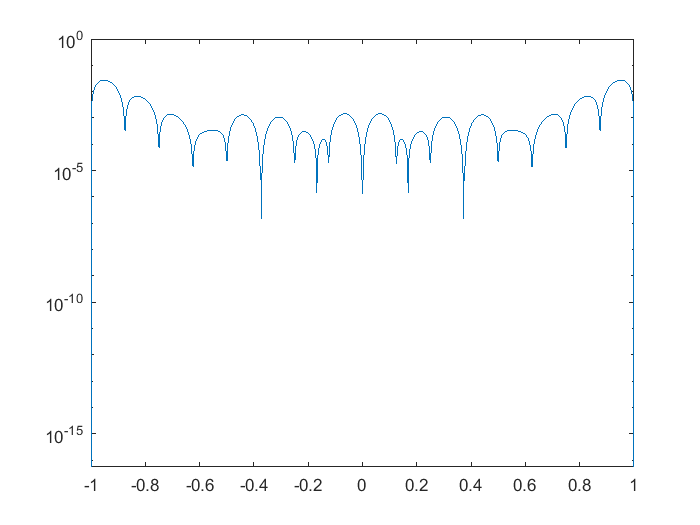
\includegraphics[scale=0.45]{hw2_1_b.png}
                        \caption{三次样条插值的逐点误差}
                    \end{figure}
              \item(15分)使用不同的 $n$, 令 $n=2^{4}, 2^{5}, \ldots, 2^{10}$ 重复上一问,取关于不同 $n$ 的2000个
                    等距点上的误差的最大值,用loglog图描述插值区
                    间上最大误差值随 $n$ 变化
                    的情况(即横轴是 $n$ )。
                    \par 解:
                    \par 本题的\textbf{MATLAB}程序显示如下:
                    \begin{lstlisting}[frame=single]
clear,clc
syms x;
F = @(x) sin(4 * (x^2)) + (sin(4 * x))^2;
err = [4:10];

for g = 4:10
    n = 2^g;
    A = eye(n + 1);
    A = 2 * A;
    A(1, 2) = 1;
    A(n + 1, n) = 1;
    h = (1 - (-1)) / n;
    lambda = 1/2;
    mu = 1 - lambda;

    for i = 2:n
        A(i, i - 1) = mu;
        A(i, i + 1) = lambda;
    end

    y = [0:1:n];
    xx = [0:1:n];

    for i = 1:n + 1
        xx(i) = -1 + (i - 1) * h;
        y(i) = F(xx(i));
    end

    d = [0:1:n];

    for i = 2:n
        d(i) = 3 * (y(i + 1) - 2 * y(i) + y(i - 1)) / (h^2);
    end

    d(1) = 6 / h * ((y(2) - y(1)) / h - 0);
    d(n + 1) = 6 / h * (0 - (y(n + 1) - y(n)) / h);
    d = d';
    M = A \ d;
    k = 1;
    xk_1 = xx(2);
    xk = xx(1);
    h_new = 2/2000;
    t = -1;
    C = y(1) / h - h * M(1) / 6;
    D = y(2) / h - h * M(2) / 6;
    error_delta = [0:1:n];

    for i = 0:2000
        t = -1 + i * h_new;

        if (t >= xk && t <= xk_1) || t > 1
            s = (xk_1 - t)^3 / (6 * h) * M(k) + (t - xk)^3 / (6 * h) * M(k + 1) + C * (xk_1 - t) + D * (t - xk);
            error_delta(i + 1) = abs(s - F(t));

        else
            k = k + 1;
            xk_1 = xx(k + 1);
            xk = xx(k);
            C = y(k) / h - h * M(k) / 6;
            D = y(k + 1) / h - h * M(k + 1) / 6;
            s = (xk_1 - t)^3 / (6 * h) * M(k) + (t - xk)^3 / (6 * h) * M(k + 1) + C * (xk_1 - t) + D * (t - xk);
            error_delta(i + 1) = abs(s - F(t));
        end

    end

    err(g - 3) = max(error_delta);
end
loglog([4:10], err);
\end{lstlisting}
                    \par 程序运行输出结果为:
                    \begin{figure}[H]
                        \centering
                        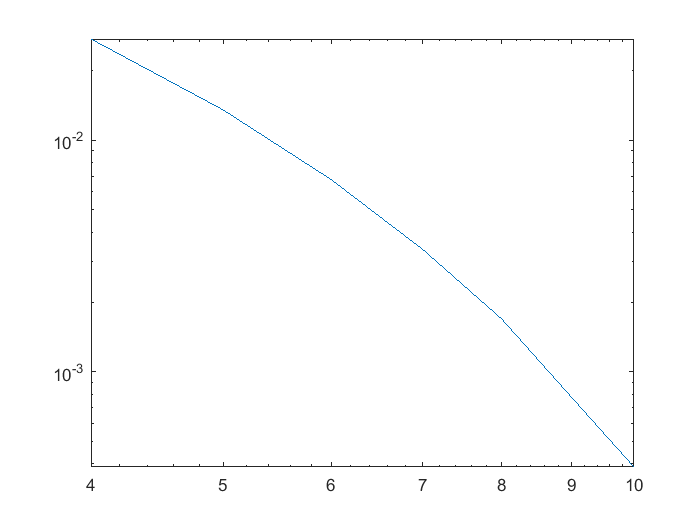
\includegraphics[scale=0.45]{hw2_1_c.png}
                        \caption{三次样条插值区
                            间上最大误差值随 $n$ 变化
                            的情况}
                    \end{figure}
              \item(15分)针对周期边界条件,即假设三次样条函数满足 $S^{\prime}(-1)=S^{\prime}(1)$ 和 $S^{\prime \prime}(-1)=$ $S^{\prime \prime}(1)$, 重复完成上面三问中的要求。
                    \par 解:
                    \par 在题设的边界条件下,\text { 由 } $S^{\prime \prime}\left(x_{0}+0\right)=S^{\prime \prime}\left(x_{n}-0\right)$ \text { 可得 } $M_{0}=M_{n}$。再由条件 $S^{\prime}\left(x_{0}+0\right)=S^{\prime}\left(x_{n}-0\right)$ 可得
                    $$
                        -M_{0} \cdot \frac{h_{1}}{2}+\frac{y_{1}-y_{0}}{h_{1}}-\frac{h_{1}}{6}\left(M_{1}-M_{0}\right)=M_{n} \cdot \frac{h_{n}}{2}+\frac{y_{n}-y_{n-1}}{h_{n}}-\frac{h_{n}}{6}\left(M_{n}-M_{n-1}\right)
                    $$
                    只要注意到 $y_{0}=y_{n}, M_{0}=M_{n}$, 整理上式即得
                    \begin{equation}\label{eq4}
                        \lambda_{n} M_{1}+\mu_{n} M_{n-1}+2 M_{n}=\frac{6}{h_{1}+h_{n}}\left(\frac{y_{1}-y_{0}}{h_{1}}-\frac{y_{n}-y_{n-1}}{h_{n}}\right)
                    \end{equation}
                    由式 \ref{eq3} 和式 \ref{eq4}, 可确定 $M_{1}, M_{2}, \cdots, M_{n}$ 的线性方程组为
                    $$
                        \left[\begin{array}{ccccc}
                                2           & \lambda_{1} &             &         & \mu_{1}       \\
                                \mu_{2}     & 2           & \lambda_{2} &         &               \\
                                            & \ddots      & \ddots      & \ddots  &               \\
                                            &             & \mu_{n-1}   & 2       & \lambda_{n-1} \\
                                \lambda_{n} &             &             & \mu_{n} & 2
                            \end{array}\right]\left[\begin{array}{c}
                                M_{1}   \\
                                M_{2}   \\
                                \vdots  \\
                                M_{n-1} \\
                                M_{n}
                            \end{array}\right]=\left[\begin{array}{c}
                                d_{1}   \\
                                d_{2}   \\
                                \vdots  \\
                                d_{n-1} \\
                                d_{n}
                            \end{array}\right]
                    $$
                    \par 本题(重复(b))的\textbf{MATLAB}程序显示如下:
                    \begin{lstlisting}[frame=single]
clear,clc
syms x;
F = @(x) sin(4 * (x^2)) + (sin(4 * x))^2;
n = 2^4;
A = eye(n);
A = 2 * A;
h = (1 - (-1)) / n;
lambda = 1/2;
mu = 1 - lambda;
A(1, 2) = lambda;
A(n, 1) = lambda;
A(1, n) = mu;
A(n, n - 1) = mu;

for i = 2:n - 1
    A(i, i - 1) = mu;
    A(i, i + 1) = lambda;
end

y = [0:1:n];
xx = [0:1:n];

for i = 1:n + 1
    xx(i) = -1 + (i - 1) * h;
    y(i) = F(xx(i));
end

d = [1:1:n];

for i = 2:n
    d(i - 1) = 3 * (y(i + 1) - 2 * y(i) + y(i - 1)) / (h^2);
end

d(n) = 6 / h * (0 - (y(n + 1) - y(n)) / h);
d = d';
M = A \ d;
tmp = M;
M(1) = tmp(n);

for i = 1:n
    M(i + 1) = tmp(i);
end

k = 1;
xk_1 = xx(2);
xk = xx(1);
h_new = 2/2000;
t = -1;
C = y(1) / h - h * M(1) / 6;
D = y(2) / h - h * M(2) / 6;
error_delta = [0:1:n];

for i = 0:2000
    t = -1 + i * h_new;

    if (t >= xk && t <= xk_1) || t > 1
        s = (xk_1 - t)^3 / (6 * h) * M(k) + (t - xk)^3 / (6 * h) * M(k + 1) + C * (xk_1 - t) + D * (t - xk);
        error_delta(i + 1) = abs(s - F(t));

    else
        k = k + 1;
        xk_1 = xx(k + 1);
        xk = xx(k);
        C = y(k) / h - h * M(k) / 6;
        D = y(k + 1) / h - h * M(k + 1) / 6;
        s = (xk_1 - t)^3 / (6 * h) * M(k) + (t - xk)^3 / (6 * h) * M(k + 1) + C * (xk_1 - t) + D * (t - xk);
        error_delta(i + 1) = abs(s - F(t));
    end

end

semilogy([-1:h_new:1], error_delta)
\end{lstlisting}
                    \par 程序运行输出结果为:
                    \begin{figure}[H]
                        \centering
                        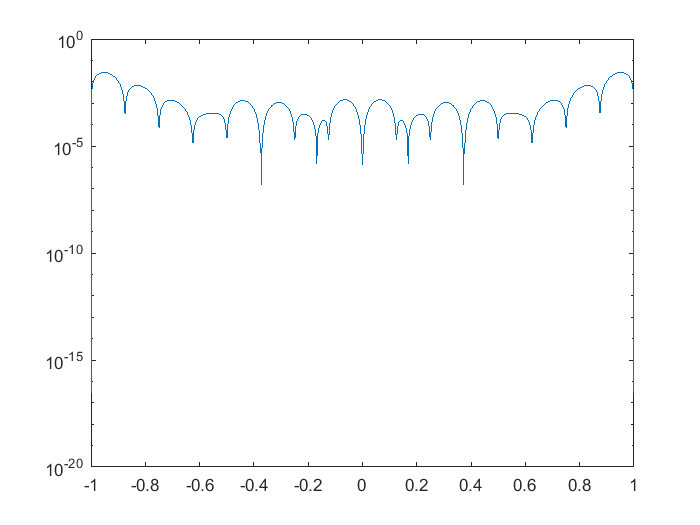
\includegraphics[scale=0.45]{hw2_1_d_1.png}
                        \caption{三次样条插值的逐点误差(周期边界条件)}
                    \end{figure}
                    \par 本题的\textbf{MATLAB}程序显示如下:
                    \begin{lstlisting}[frame=single]
clear,clc
syms x;
F = @(x) sin(4 * (x^2)) + (sin(4 * x))^2;
err = [4:10];

for g = 4:10
    n = 2^g;
    A = eye(n);
    A = 2 * A;
    h = (1 - (-1)) / n;
    lambda = 1/2;
    mu = 1 - lambda;
    A(1, 2) = lambda;
    A(n, 1) = lambda;
    A(1, n) = mu;
    A(n, n - 1) = mu;

    for i = 2:n - 1
        A(i, i - 1) = mu;
        A(i, i + 1) = lambda;
    end

    y = [0:1:n];
    xx = [0:1:n];

    for i = 1:n + 1
        xx(i) = -1 + (i - 1) * h;
        y(i) = F(xx(i));
    end

    d = [1:1:n];

    for i = 2:n
        d(i - 1) = 3 * (y(i + 1) - 2 * y(i) + y(i - 1)) / (h^2);
    end

    d(n) = 6 / h * (0 - (y(n + 1) - y(n)) / h);
    d = d';
    M = A \ d;
    tmp = M;
    M(1) = tmp(n);

    for i = 1:n
        M(i + 1) = tmp(i);
    end

    k = 1;
    xk_1 = xx(2);
    xk = xx(1);
    h_new = 2/2000;
    t = -1;
    C = y(1) / h - h * M(1) / 6;
    D = y(2) / h - h * M(2) / 6;
    error_delta = [0:1:n];

    for i = 0:2000
        t = -1 + i * h_new;

        if (t >= xk && t <= xk_1) || t > 1
            s = (xk_1 - t)^3 / (6 * h) * M(k) + (t - xk)^3 / (6 * h) * M(k + 1) + C * (xk_1 - t) + D * (t - xk);
            error_delta(i + 1) = abs(s - F(t));

        else
            k = k + 1;
            xk_1 = xx(k + 1);
            xk = xx(k);
            C = y(k) / h - h * M(k) / 6;
            D = y(k + 1) / h - h * M(k + 1) / 6;
            s = (xk_1 - t)^3 / (6 * h) * M(k) + (t - xk)^3 / (6 * h) * M(k + 1) + C * (xk_1 - t) + D * (t - xk);
            error_delta(i + 1) = abs(s - F(t));
        end

    end

    err(g - 3) = max(error_delta);
end

loglog([4:10], err);
\end{lstlisting}
                    \par 程序运行输出结果为:
                    \begin{figure}[H]
                        \centering
                        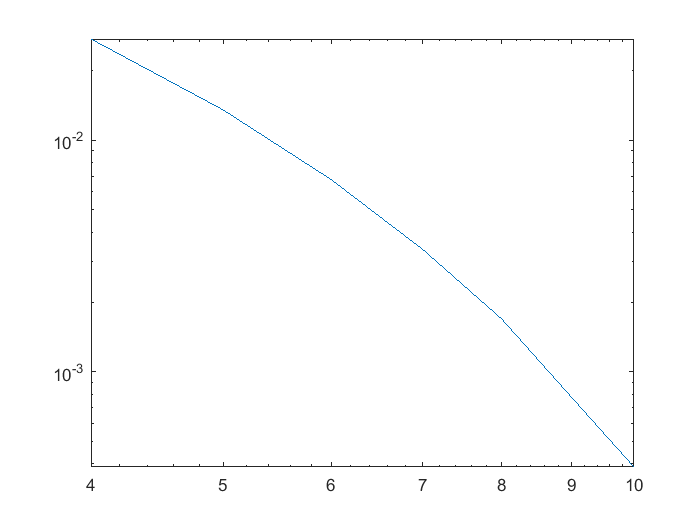
\includegraphics[scale=0.45]{hw2_1_c.png}
                        \caption{三次样条插值区
                            间上最大误差值随 $n$ 变化
                            的情况(周期边界条件)}
                    \end{figure}
          \end{enumerate}
    \item[第二题] 本题深入讨论Newton插值公式的性质。
          \begin{enumerate}\item(15分) 对于一个光滑函数 $f(x)$, 证明若 $\left\{i_{0}, i_{1}, \ldots, i_{k}\right\}$ 是 $\{0,1, \ldots, k\}$ 的任意一 个排列,则
                    $$
                        f\left[x_{0}, x_{1}, \ldots, x_{k}\right]=f\left[x_{i_{0}}, x_{i_{1}}, \ldots, x_{i_{k}}\right]
                    $$
                    \par 证:
                    \par 先证引理:$k$ 阶差商 $f\left[x_{0}, x_{1}, \cdots, x_{k}\right]$ 是由函数值 $f\left(x_{0}\right), f\left(x_{1}\right), \cdots, f\left(x_{k}\right)$的
                    线性组合而成.
                    $$
                        f\left[x_{0}, x_{1}, \cdots, x_{k}\right]=\sum_{i=0}^{k} \frac{1}{\left(x_{i}-x_{0}\right) \cdots\left(x_{i}-x_{i-1}\right)\left(x_{i}-x_{i+1}\right) \cdots\left(x_{i}-x_{k}\right)} f\left(x_{i}\right)
                    $$
                    用归纳法可以证明这一引理。
                    \par 显然,当$k=1$时,引理成立。
                    \par 假设当$k=n-1$时,引理成立,故有:
                    $$f\left[x_{0}, x_{1}, \cdots, x_{n-1}\right]=\sum_{i=0}^{n-1} \frac{1}{\left(x_{i}-x_{0}\right) \cdots\left(x_{i}-x_{i-1}\right)\left(x_{i}-x_{i+1}\right) \cdots\left(x_{i}-x_{n-1}\right)} f\left(x_{i}\right)$$
                    $$f\left[x_{1}, x_{2},\cdots, x_{n}\right]=\sum_{i=1}^{n} \frac{1}{\left(x_{i}-x_{1}\right) \cdots\left(x_{i}-x_{i-1}\right)\left(x_{i}-x_{i+1}\right) \cdots\left(x_{i}-x_{n}\right)} f\left(x_{i}\right)$$
                    \par 则$k=n$时:
                    $$
                        \begin{aligned}
                            f\left[x_{0}, x_{1}, \cdots, x_{n}\right] & =\frac{f\left[x_{0}, x_{1}, \cdots, x_{n-1}\right]-f\left[x_{1}, x_{2},\cdots, x_{n}\right]}{x_{0}-x_{n}}                                                        \\
                                                                      & =\sum_{i=0}^{k} \frac{1}{\left(x_{i}-x_{0}\right) \cdots\left(x_{i}-x_{i-1}\right)\left(x_{i}-x_{i+1}\right) \cdots\left(x_{i}-x_{n}\right)} f\left(x_{i}\right)\end{aligned}
                    $$
                    \par 引理证毕,故有:
                    $$
                        f\left[x_{0}, x_{1}, \cdots, x_{k}\right]=\sum_{i=0}^{k} \frac{1}{\left(x_{i}-x_{0}\right) \cdots\left(x_{i}-x_{i-1}\right)\left(x_{i}-x_{i+1}\right) \cdots\left(x_{i}-x_{k}\right)} f\left(x_{i}\right)
                    $$
                    $$
                        f\left[x_{i_{0}}, x_{i_{1}}, \cdots, x_{i_{k}}\right]=\sum_{j=0}^{k} \frac{1}{\left(x_{i_{j}}-x_{i_{0}}\right) \cdots\left(x_{i_{j}}-x_{i_{j-1}}\right)\left(x_{i_{j}}-x_{i_{j+1}}\right) \cdots\left(x_{i_{j}}-x_{i_{k}}\right)} f\left(x_{i_{j}}\right)
                    $$
                    \par 又因$\{x_{0}, x_{1}, \cdots, x_{k}\}$与$\{x_{i_{0}}, x_{i_{1}}, \cdots, x_{i_{k}}\}$之间存在双射,易得:
                    $$
                        f\left[x_{0}, x_{1}, \ldots, x_{k}\right]=f\left[x_{i_{0}}, x_{i_{1}}, \ldots, x_{i_{k}}\right]
                    $$
              \item (10分)课堂上我们提到了Chebyshev点
                    $$
                        x_{j}=\cos (j \pi / n) \quad j=0,1, \ldots, n
                    $$
                    以及使用Chebyshev点可以有效地克服Runge现象。写一个\textbf{MATLAB}程序,令 $n=2^{2}, 2^{3}, 2^{4}, \ldots, 2^{7}$, 按照从右到左的顺序(即 $j$ 从小到大的顺序)使用对应
                    的 $n+1$ 个Chebyshev点对定义在 $[-1,1]$ 上的Runge函数
                    $$
                        f(x)=\frac{1}{1+25 x^{2}}
                    $$
                    进行插值,并取2000个等距点上的误差的最大值,用semilogy图描述插值区
                    间上最大误差值随 $n$ 变化的情况(即横轴是 $n$) 。
                    \par 解:
                    \par 本题的\textbf{MATLAB}程序显示如下:
                    \begin{lstlisting}[frame=single]
clear,clc

syms x;
F = @(x) 1 / (1 + 25 * x^2);
y = [0:1:2000];

for i = 0:2000
    y(i + 1) = F(-1 + i * 2/2000);
end

result = [0:1:2000];
delta_result = [2:1:7];

for n = 2:7
    count = 2^n;
    chebyshev = [0:1:count];

    for j = 0:1:count
        chebyshev(j + 1) = cos(j * pi / (count));
    end

    d_f = [1:1:count];
    g = [0:1:count];

    for i = 1:count + 1
        g(i) = F(chebyshev(i));
    end

    for k = 2:count + 1

        for i = count + 1:-1:k
            g(i) = (g(i) - g(i - 1)) / (chebyshev(i) - chebyshev(i - k + 1));
        end

    end

    for i = 0:2000
        a = -1 + i * 2/2000;
        result(i + 1) = F(chebyshev(1));

        for j = 1:count
            tmp = 1;

            for k = 1:j
                tmp = tmp * (a - chebyshev(k));
            end

            result(i + 1) = result(i + 1) + tmp * g(j + 1);
        end

    end

    tmp = [0:1:2000];

    for i = 0:2000
        tmp(i + 1) = abs(result(i + 1) - y(i + 1));
    end

    delta_result(n - 1) = max(tmp);
end

semilogy([2:7], delta_result);
\end{lstlisting}
                    \par 程序运行输出结果为:
                    \begin{figure}[H]
                        \centering
                        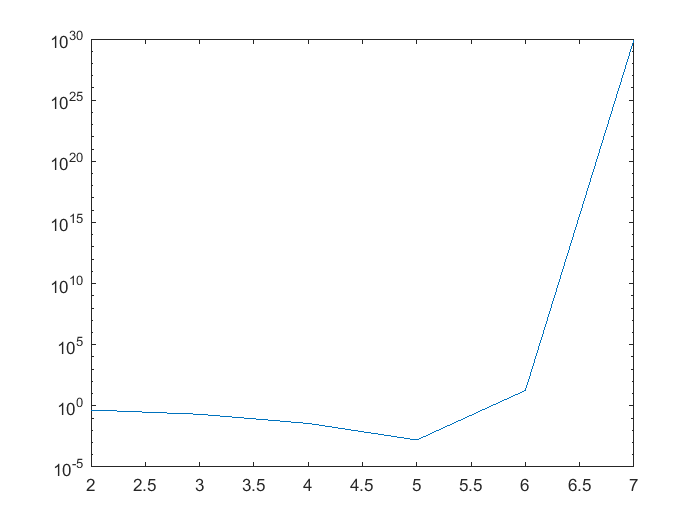
\includegraphics[scale=0.45]{hw2_2_b.png}
                        \caption{Newton插值区间上误差值随n变化的情况(Chebyshev点按从左到右顺序使用)}
                    \end{figure}

              \item (10分) 重复上一问,但使用随机数种子rng(22)和randperm函数来随机计算 差商时插值点的使用顺序,取关于不同 $n$ 的2000个等距点上的误差的最大值,
                    用semilogy图描述插值区间上最大误差值随 $n$ 变化的情况(即横轴是 $n$) 。
                    \par 解:
                    \par 本题的\textbf{MATLAB}程序显示如下:
                    \begin{lstlisting}[frame=single]
clear,clc

syms x;
F = @(x) 1 / (1 + 25 * x^2);
y = [0:1:2000];

for i = 0:2000
    y(i + 1) = F(-1 + i * 2/2000);
end

result = [0:1:2000];
delta_result = [2:1:7];

for n = 2:7
    count = 2^n;
    chebyshev = [0:1:count];
    rng(22);
    r = randperm(count + 1);

    for j = 1:1:count + 1
        chebyshev(j) = cos((r(j) - 1) * pi / (count));
    end

    d_f = [1:1:count];
    g = [0:1:count];

    for i = 1:count + 1
        g(i) = F(chebyshev(i));
    end

    for k = 2:count + 1

        for i = count + 1:-1:k
            g(i) = (g(i) - g(i - 1)) / (chebyshev(i) - chebyshev(i - k + 1));
        end

    end

    for i = 0:2000
        a = -1 + i * 2/2000;
        result(i + 1) = F(chebyshev(1));

        for j = 1:count
            tmp = 1;

            for k = 1:j
                tmp = tmp * (a - chebyshev(k));
            end

            result(i + 1) = result(i + 1) + tmp * g(j + 1);
        end

    end

    tmp = [0:1:2000];

    for i = 0:2000
        tmp(i + 1) = abs(result(i + 1) - y(i + 1));
    end

    delta_result(n - 1) = max(tmp);
end

semilogy([2:7], delta_result);
\end{lstlisting}
                    \par 程序运行输出结果为:
                    \begin{figure}[H]
                        \centering
                        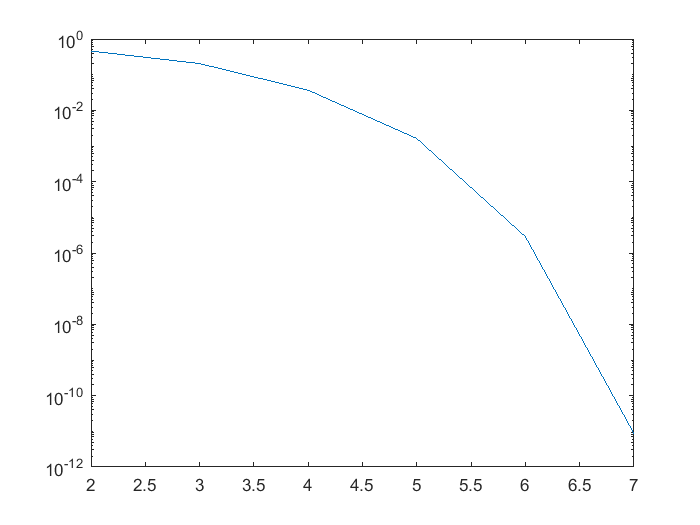
\includegraphics[scale=0.45]{hw2_2_c.png}
                        \caption{Newton插值区间上误差值随n变化的情况(Chebyshev点按随机顺序使用)}
                    \end{figure}
              \item(10分)试着解释上面两小问中你观察到的不同现象产生的原因。注: 此问
                    答不出来也无妨。
                    \par 解:
                    \par 由Newton插值多项式的余项公式:$$
                        R(x)=\frac{f^{(n+1)}(\xi)}{(n+1) !} \prod_{i=0}^{n}\left(x-x_{i}\right)=f\left[x, x_{0}, \cdots, x_{n}\right] \prod_{i=0}^{n}\left(x-x_{i}\right)
                    $$
                    \par 结合公式:
                    $$
                        f\left[x_{0}, x_{1}, \ldots, x_{k}\right]=f\left[x_{i_{0}}, x_{i_{1}}, \ldots, x_{i_{k}}\right]
                    $$
                    \par 可以推断,Newton插值的余项大小与插值点的使用顺序无关。
                    \par 但在本题中,Chebyshev点分别按顺序使用和乱序使用,得到的Newton插值结果差异较大。可能的原因是:在计算差商的过程中,需要反复除以区间长度。Chebyshev点间的区间长度随着n的增大,而不断减小。在顺序使用的过程中,除以的区间长度也不断减小。
                    但随着区间长度变小,误差随之增大,且多次计算后,误差累积放大。而乱序使用Chebyshev点,则能够减少区间长度过小的情况出现,减小了因为机器精度等因素带来的影响。

          \end{enumerate}
    \item[第三题] 本题用于讨论周期函数的Lagrange插值方法。对于周期函数而言,多项式不再是 最有效的基函数,而等距插值点也不再会出现Runge现象。逼近周期函数的基函 数通常选用三角函数或者复指数。同时注意对于周期函数而言,插值点数量和子
          区间个数相等。
          \begin{enumerate}\item (10分)在 $[0,1]$ 上关于周期函数的基于等间距插值点 $x_{j}=\frac{j}{n}, j=0,1, \ldots$, $n-1$ 的Lagrange插值基函数为
                    $$
                        \ell_{k}(x)=\left\{\begin{array}{ll}
                            \frac{(-1)^{k}}{n} \sin (n \pi x) \csc \left(\pi\left(x-x_{k}\right)\right) & \text { 若 } n \text { 为奇数 } \\
                            \frac{(-1)^{k}}{n} \sin (n \pi x) \cot \left(\pi\left(x-x_{k}\right)\right) & \text { 若 } n \text { 为偶数 }
                        \end{array}\right.
                    $$
                    证明对于 $n$ 分别为奇数和偶数的情况下
                    $$
                        \ell_{k}\left(x_{j}\right)=\left\{\begin{array}{ll}
                            1 & k=j      \\
                            0 & k \neq j
                        \end{array}\right.
                    $$
                    \par 证:
                    \par 当$n$ 为奇数时:
                    \par $$\ell_{k}\left(x_{j}\right)=\frac{(-1)^{k}}{n} \sin (n \pi x_{j}) \csc \left(\pi\left(x_{j}-x_{k}\right)\right)$$
                    \par 将$x_{j}=\frac{j}{n},x_{k}=\frac{k}{n}$代入得:
                    \par $$\ell_{k}\left(x_{j}\right)=\frac{(-1)^{k}}{n} \sin (j \pi ) \csc \left(\frac{\pi}{n}\left(j-k\right)\right)$$
                    \par 当$k \neq j$时,$\sin (j \pi )=0,\csc \left(\frac{\pi}{n}\left(j-k\right)\right)\neq 0$,故得:
                    $$\ell_{k}\left(x_{j}\right)=0,k \neq j,n \text { 为奇数 }$$
                    \par 当$k=j$时,$\sin (j \pi )=0,\sin \left(\frac{\pi}{n}\left(j-k\right)\right)= 0$,故有:
                    $$\begin{aligned}\ell_{k}\left(x_{j}\right) & =\frac{(-1)^{k}}{n} \sin (j \pi ) \csc \left(\frac{\pi}{n}\left(j-k\right)\right)                                   \\
                                                       & =\lim_{x \to x_{k}}\frac{(-1)^{k}}{n} \sin (n \pi x) \csc \left(\pi\left(x-x_{k}\right)\right)                      \\
                                                       & =\lim_{j \to k}  \frac{(-1)^{k}}{n} \sin (j \pi ) \csc \left(\frac{\pi}{n}\left(j-k\right)\right)                   \\
                                                       & =\lim_{j \to k}\frac{(-1)^{k}}{n} \frac{\sin (j \pi )}{ \sin \left(\frac{\pi}{n}\left(j-k\right)\right)}            \\
                                                       & =\frac{(-1)^{k}}{n}\lim_{j \to k}\frac{\pi \cos(j\pi)}{\frac{\pi}{n}\cos\left(\frac{\pi}{n}\left(j-k\right)\right)} \\
                                                       & =\frac{(-1)^{k}}{n}\frac{\pi \cos(k\pi)}{\frac{\pi}{n}\cos\left(0\right)}                                           \\
                                                       & =1
                        \end{aligned}
                    $$
                    \par 即:
                    $$\ell_{k}\left(x_{j}\right)=1,k = j,n \text { 为奇数 }$$
                    \par 当$n$ 为偶数时:
                    \par $$\ell_{k}\left(x_{j}\right)=\frac{(-1)^{k}}{n} \sin (n \pi x_{j}) \cot \left(\pi\left(x_{j}-x_{k}\right)\right)$$
                    \par 将$x_{j}=\frac{j}{n},x_{k}=\frac{k}{n}$代入得:
                    \par $$\ell_{k}\left(x_{j}\right)=\frac{(-1)^{k}}{n} \sin (j \pi ) \cot \left(\frac{\pi}{n}\left(j-k\right)\right)$$
                    \par 当$k \neq j$时,$\sin (j \pi )=0,\cot \left(\frac{\pi}{n}\left(j-k\right)\right)\neq 0$,故得:
                    $$\ell_{k}\left(x_{j}\right)=0,k \neq j, n \text { 为偶数 }$$
                    \par 当$k=j$时,$\sin (j \pi )=0,\sin \left(\frac{\pi}{n}\left(j-k\right)\right)= 0$,故有:
                    $$\begin{aligned}\ell_{k}\left(x_{j}\right) & =\frac{(-1)^{k}}{n} \sin (j \pi ) \cot \left(\frac{\pi}{n}\left(j-k\right)\right)                                                                                               \\
                                                       & =\lim_{x \to x_{k}}\frac{(-1)^{k}}{n} \sin (n \pi x) \cot \left(\pi\left(x-x_{k}\right)\right)                                                                                  \\
                                                       & =\lim_{j \to k}  \frac{(-1)^{k}}{n} \sin (j \pi ) \cot \left(\frac{\pi}{n}\left(j-k\right)\right)                                                                               \\
                                                       & =\lim_{j \to k}\frac{(-1)^{k}}{n}\cos\left(\frac{\pi}{n}\left(j-k\right)\right) \frac{\sin (j \pi )}{ \sin \left(\frac{\pi}{n}\left(j-k\right)\right)}                          \\
                                                       & =\frac{(-1)^{k}}{n}\lim_{j \to k}\cos\left(\frac{\pi}{n}\left(j-k\right)\right)\lim_{j \to k}\frac{\pi \cos(j\pi)}{\frac{\pi}{n}\cos\left(\frac{\pi}{n}\left(j-k\right)\right)} \\
                                                       & =\frac{(-1)^{k}}{n}\frac{\pi \cos(k\pi)}{\frac{\pi}{n}\cos\left(0\right)}                                                                                                       \\
                                                       & =1
                        \end{aligned}
                    $$
                    \par 即:
                    $$\ell_{k}\left(x_{j}\right)=1,k = j,n \text { 为偶数 }$$
                    \par 综上:
                    $$
                        \ell_{k}\left(x_{j}\right)=\left\{\begin{array}{ll}
                            1 & k=j      \\
                            0 & k \neq j
                        \end{array}\right.
                    $$
              \item (10分)用上述对应于 $n$ 为偶数的Lagrange基函数构造Lagrange插值多项式. 并用 $n=2^{6}$ 个点对周期函数 $f(x)=\sin (2 \pi x) e^{\cos (2 \pi x)}$ 在 $[0,1]$ 上进行插值。取1000个 等距点上的误差,用semilogy图描述插值区间上误差值随 $x$ 变化的情况(即
                    横轴是 $x$ )。
                    \par 解:
                    \par 本题的\textbf{MATLAB}程序显示如下:
                    \begin{lstlisting}[frame=single]
clear,clc
syms x;
syms k;
n = 2^6;
F = @(x) sin(2 * pi * x) * exp(cos(2 * pi * x));
l = @(x, k) ((-1)^k) / n * sin(n * pi * x) * cot(pi * (x - k / n));
result=[0:1:1999];
y=[0:1:1999];
delta_y=[0:1:1999];
for i=0:1999
    y(i+1)=F(i/2000);
    tmp=0;

    for j=0:n-1
        tmp=tmp+l(i/2000,j)*F(j/n);
    end
    result(i+1)=tmp;
    delta_y(i+1)=abs(result(i+1)-y(i+1));
end
x=[0:1/2000:1-1/2000];
semilogy(x,delta_y)
\end{lstlisting}
                    \par 程序运行输出结果为:
                    \begin{figure}[H]
                        \centering
                        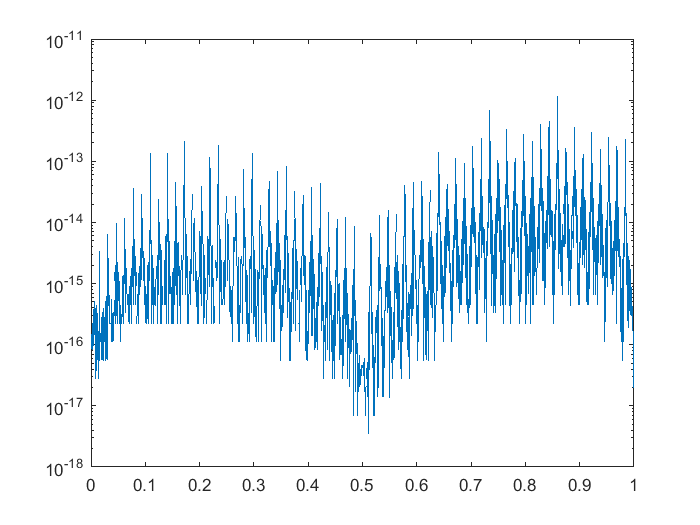
\includegraphics[scale=0.45]{hw2_3.png}
                        \caption{Lagrange插值区间上误差值随x变化的情况}
                    \end{figure}
          \end{enumerate}
    \item[第四题] (10分) 写程序完成课本 59 页第7题,并计算出你的拟合函数对比所给数据点的
          误差的2-范数。
          \par 解:
          \par 作有理函数拟合 $\varphi(x)=\frac{a_{0}+a_{1} x+\cdots+a_{p} x^{p}}{1+b_{1} x+\cdots+b_{q} x^{q}}$, 可令
          $$
              Q=\sum_{i=1}^{m}\left(a_{0}+a_{1} x_{i}+\cdots+a_{p} x_{i}^{p}-b_{1} x_{i} y_{i}-\cdots-b_{q} x_{i}^{q} y_{i}-y_{i}\right)^{2}
          $$
          \par 本题中$\varphi(x)=\frac{a_{1}}{1+b_{1} x}$,故
          $$
              Q=\sum_{i=1}^{m}\left(a_{1} x_{i}-b_{1} x_{i} y_{i}\right)^{2}$$
          \par 本题的\textbf{MATLAB}程序显示如下:
          \begin{lstlisting}[frame=single]
clc, clear
x = [2.1, 2.5, 2.8, 3.2];
y = [0.6087, 0.6849, 0.7368, 0.8111];
a_1 = 0;
b_1 = 0;
x_y = x .* y;
c_11 = sum(x .* x);
c_12 = -sum(x .* x_y);
c_21 = -c_12;
c_22 = -sum(x_y .* x_y);
B_1 = sum(x .* y);
B_2 = sum(x_y .* y);
C = [c_11, c_12; c_21, c_22];
B = [B_1; B_2];
tmp = C \ B;
a_1 = tmp(1);
b_1 = tmp(2);
a = 1 / a_1;
b = b_1 / a_1;
y_bar = [Phi(x(1), a, b), Phi(x(2), a, b), Phi(x(3), a, b), Phi(x(4), a, b)];
delta_y = y - y_bar;
X = sprintf('The 2-norm of the error of the fitting function compared to the given data point is %.15f', norm(delta_y, 2));
disp(X)

function value = Phi(x, a, b)
    value = x / (a + b * x);
end

\end{lstlisting}
          \par 程序运行输出结果为:
          \begin{lstlisting}[frame=single]
The 2-norm of the error of the fitting function compared to the given data point is 0.005738349475781
\end{lstlisting}
\end{enumerate}




\end{document}
